% Options for packages loaded elsewhere
\PassOptionsToPackage{unicode}{hyperref}
\PassOptionsToPackage{hyphens}{url}
\PassOptionsToPackage{dvipsnames,svgnames,x11names}{xcolor}
%
\documentclass[
  letterpaper,
]{krantz}

\usepackage{amsmath,amssymb}
\usepackage{iftex}
\ifPDFTeX
  \usepackage[T1]{fontenc}
  \usepackage[utf8]{inputenc}
  \usepackage{textcomp} % provide euro and other symbols
\else % if luatex or xetex
  \usepackage{unicode-math}
  \defaultfontfeatures{Scale=MatchLowercase}
  \defaultfontfeatures[\rmfamily]{Ligatures=TeX,Scale=1}
\fi
\usepackage{lmodern}
\ifPDFTeX\else  
    % xetex/luatex font selection
\fi
% Use upquote if available, for straight quotes in verbatim environments
\IfFileExists{upquote.sty}{\usepackage{upquote}}{}
\IfFileExists{microtype.sty}{% use microtype if available
  \usepackage[]{microtype}
  \UseMicrotypeSet[protrusion]{basicmath} % disable protrusion for tt fonts
}{}
\makeatletter
\@ifundefined{KOMAClassName}{% if non-KOMA class
  \IfFileExists{parskip.sty}{%
    \usepackage{parskip}
  }{% else
    \setlength{\parindent}{0pt}
    \setlength{\parskip}{6pt plus 2pt minus 1pt}}
}{% if KOMA class
  \KOMAoptions{parskip=half}}
\makeatother
\usepackage{xcolor}
\setlength{\emergencystretch}{3em} % prevent overfull lines
\setcounter{secnumdepth}{5}
% Make \paragraph and \subparagraph free-standing
\ifx\paragraph\undefined\else
  \let\oldparagraph\paragraph
  \renewcommand{\paragraph}[1]{\oldparagraph{#1}\mbox{}}
\fi
\ifx\subparagraph\undefined\else
  \let\oldsubparagraph\subparagraph
  \renewcommand{\subparagraph}[1]{\oldsubparagraph{#1}\mbox{}}
\fi

\usepackage{color}
\usepackage{fancyvrb}
\newcommand{\VerbBar}{|}
\newcommand{\VERB}{\Verb[commandchars=\\\{\}]}
\DefineVerbatimEnvironment{Highlighting}{Verbatim}{commandchars=\\\{\}}
% Add ',fontsize=\small' for more characters per line
\usepackage{framed}
\definecolor{shadecolor}{RGB}{241,243,245}
\newenvironment{Shaded}{\begin{snugshade}}{\end{snugshade}}
\newcommand{\AlertTok}[1]{\textcolor[rgb]{0.68,0.00,0.00}{#1}}
\newcommand{\AnnotationTok}[1]{\textcolor[rgb]{0.37,0.37,0.37}{#1}}
\newcommand{\AttributeTok}[1]{\textcolor[rgb]{0.40,0.45,0.13}{#1}}
\newcommand{\BaseNTok}[1]{\textcolor[rgb]{0.68,0.00,0.00}{#1}}
\newcommand{\BuiltInTok}[1]{\textcolor[rgb]{0.00,0.23,0.31}{#1}}
\newcommand{\CharTok}[1]{\textcolor[rgb]{0.13,0.47,0.30}{#1}}
\newcommand{\CommentTok}[1]{\textcolor[rgb]{0.37,0.37,0.37}{#1}}
\newcommand{\CommentVarTok}[1]{\textcolor[rgb]{0.37,0.37,0.37}{\textit{#1}}}
\newcommand{\ConstantTok}[1]{\textcolor[rgb]{0.56,0.35,0.01}{#1}}
\newcommand{\ControlFlowTok}[1]{\textcolor[rgb]{0.00,0.23,0.31}{#1}}
\newcommand{\DataTypeTok}[1]{\textcolor[rgb]{0.68,0.00,0.00}{#1}}
\newcommand{\DecValTok}[1]{\textcolor[rgb]{0.68,0.00,0.00}{#1}}
\newcommand{\DocumentationTok}[1]{\textcolor[rgb]{0.37,0.37,0.37}{\textit{#1}}}
\newcommand{\ErrorTok}[1]{\textcolor[rgb]{0.68,0.00,0.00}{#1}}
\newcommand{\ExtensionTok}[1]{\textcolor[rgb]{0.00,0.23,0.31}{#1}}
\newcommand{\FloatTok}[1]{\textcolor[rgb]{0.68,0.00,0.00}{#1}}
\newcommand{\FunctionTok}[1]{\textcolor[rgb]{0.28,0.35,0.67}{#1}}
\newcommand{\ImportTok}[1]{\textcolor[rgb]{0.00,0.46,0.62}{#1}}
\newcommand{\InformationTok}[1]{\textcolor[rgb]{0.37,0.37,0.37}{#1}}
\newcommand{\KeywordTok}[1]{\textcolor[rgb]{0.00,0.23,0.31}{#1}}
\newcommand{\NormalTok}[1]{\textcolor[rgb]{0.00,0.23,0.31}{#1}}
\newcommand{\OperatorTok}[1]{\textcolor[rgb]{0.37,0.37,0.37}{#1}}
\newcommand{\OtherTok}[1]{\textcolor[rgb]{0.00,0.23,0.31}{#1}}
\newcommand{\PreprocessorTok}[1]{\textcolor[rgb]{0.68,0.00,0.00}{#1}}
\newcommand{\RegionMarkerTok}[1]{\textcolor[rgb]{0.00,0.23,0.31}{#1}}
\newcommand{\SpecialCharTok}[1]{\textcolor[rgb]{0.37,0.37,0.37}{#1}}
\newcommand{\SpecialStringTok}[1]{\textcolor[rgb]{0.13,0.47,0.30}{#1}}
\newcommand{\StringTok}[1]{\textcolor[rgb]{0.13,0.47,0.30}{#1}}
\newcommand{\VariableTok}[1]{\textcolor[rgb]{0.07,0.07,0.07}{#1}}
\newcommand{\VerbatimStringTok}[1]{\textcolor[rgb]{0.13,0.47,0.30}{#1}}
\newcommand{\WarningTok}[1]{\textcolor[rgb]{0.37,0.37,0.37}{\textit{#1}}}

\providecommand{\tightlist}{%
  \setlength{\itemsep}{0pt}\setlength{\parskip}{0pt}}\usepackage{longtable,booktabs,array}
\usepackage{calc} % for calculating minipage widths
% Correct order of tables after \paragraph or \subparagraph
\usepackage{etoolbox}
\makeatletter
\patchcmd\longtable{\par}{\if@noskipsec\mbox{}\fi\par}{}{}
\makeatother
% Allow footnotes in longtable head/foot
\IfFileExists{footnotehyper.sty}{\usepackage{footnotehyper}}{\usepackage{footnote}}
\makesavenoteenv{longtable}
\usepackage{graphicx}
\makeatletter
\def\maxwidth{\ifdim\Gin@nat@width>\linewidth\linewidth\else\Gin@nat@width\fi}
\def\maxheight{\ifdim\Gin@nat@height>\textheight\textheight\else\Gin@nat@height\fi}
\makeatother
% Scale images if necessary, so that they will not overflow the page
% margins by default, and it is still possible to overwrite the defaults
% using explicit options in \includegraphics[width, height, ...]{}
\setkeys{Gin}{width=\maxwidth,height=\maxheight,keepaspectratio}
% Set default figure placement to htbp
\makeatletter
\def\fps@figure{htbp}
\makeatother
\newlength{\cslhangindent}
\setlength{\cslhangindent}{1.5em}
\newlength{\csllabelwidth}
\setlength{\csllabelwidth}{3em}
\newlength{\cslentryspacingunit} % times entry-spacing
\setlength{\cslentryspacingunit}{\parskip}
\newenvironment{CSLReferences}[2] % #1 hanging-ident, #2 entry spacing
 {% don't indent paragraphs
  \setlength{\parindent}{0pt}
  % turn on hanging indent if param 1 is 1
  \ifodd #1
  \let\oldpar\par
  \def\par{\hangindent=\cslhangindent\oldpar}
  \fi
  % set entry spacing
  \setlength{\parskip}{#2\cslentryspacingunit}
 }%
 {}
\usepackage{calc}
\newcommand{\CSLBlock}[1]{#1\hfill\break}
\newcommand{\CSLLeftMargin}[1]{\parbox[t]{\csllabelwidth}{#1}}
\newcommand{\CSLRightInline}[1]{\parbox[t]{\linewidth - \csllabelwidth}{#1}\break}
\newcommand{\CSLIndent}[1]{\hspace{\cslhangindent}#1}

\usepackage{booktabs}
\usepackage{longtable}
\usepackage[bf,singlelinecheck=off]{caption}
\usepackage[scale=.8]{sourcecodepro}
\usepackage{hyperref}

\usepackage{framed,color}
\definecolor{shadecolor}{RGB}{248,248,248}

\renewcommand{\textfraction}{0.05}
\renewcommand{\topfraction}{0.8}
\renewcommand{\bottomfraction}{0.8}
\renewcommand{\floatpagefraction}{0.75}

\renewenvironment{quote}{\begin{VF}}{\end{VF}}
\let\oldhref\href
\renewcommand{\href}[2]{#2\footnote{\url{#1}}}

\makeatletter
\newenvironment{kframe}{%
\medskip{}
\setlength{\fboxsep}{.8em}
 \def\at@end@of@kframe{}%
 \ifinner\ifhmode%
  \def\at@end@of@kframe{\end{minipage}}%
  \begin{minipage}{\columnwidth}%
 \fi\fi%
 \def\FrameCommand##1{\hskip\@totalleftmargin \hskip-\fboxsep
 \colorbox{shadecolor}{##1}\hskip-\fboxsep
     % There is no \\@totalrightmargin, so:
     \hskip-\linewidth \hskip-\@totalleftmargin \hskip\columnwidth}%
 \MakeFramed {\advance\hsize-\width
   \@totalleftmargin\z@ \linewidth\hsize
   \@setminipage}}%
 {\par\unskip\endMakeFramed%
 \at@end@of@kframe}
\makeatother

\renewenvironment{Shaded}{\begin{kframe}}{\end{kframe}}

\usepackage{makeidx}
\makeindex

\urlstyle{tt}

\usepackage{amsthm}
\makeatletter
\def\thm@space@setup{%
  \thm@preskip=8pt plus 2pt minus 4pt
  \thm@postskip=\thm@preskip
}
\makeatother

\frontmatter
\makeatletter
\makeatother
\makeatletter
\@ifpackageloaded{bookmark}{}{\usepackage{bookmark}}
\makeatother
\makeatletter
\@ifpackageloaded{caption}{}{\usepackage{caption}}
\AtBeginDocument{%
\ifdefined\contentsname
  \renewcommand*\contentsname{Table of contents}
\else
  \newcommand\contentsname{Table of contents}
\fi
\ifdefined\listfigurename
  \renewcommand*\listfigurename{List of Figures}
\else
  \newcommand\listfigurename{List of Figures}
\fi
\ifdefined\listtablename
  \renewcommand*\listtablename{List of Tables}
\else
  \newcommand\listtablename{List of Tables}
\fi
\ifdefined\figurename
  \renewcommand*\figurename{Figure}
\else
  \newcommand\figurename{Figure}
\fi
\ifdefined\tablename
  \renewcommand*\tablename{Table}
\else
  \newcommand\tablename{Table}
\fi
}
\@ifpackageloaded{float}{}{\usepackage{float}}
\floatstyle{ruled}
\@ifundefined{c@chapter}{\newfloat{codelisting}{h}{lop}}{\newfloat{codelisting}{h}{lop}[chapter]}
\floatname{codelisting}{Listing}
\newcommand*\listoflistings{\listof{codelisting}{List of Listings}}
\makeatother
\makeatletter
\@ifpackageloaded{caption}{}{\usepackage{caption}}
\@ifpackageloaded{subcaption}{}{\usepackage{subcaption}}
\makeatother
\makeatletter
\@ifpackageloaded{tcolorbox}{}{\usepackage[skins,breakable]{tcolorbox}}
\makeatother
\makeatletter
\@ifundefined{shadecolor}{\definecolor{shadecolor}{rgb}{.97, .97, .97}}
\makeatother
\makeatletter
\makeatother
\makeatletter
\makeatother
\ifLuaTeX
  \usepackage{selnolig}  % disable illegal ligatures
\fi
\IfFileExists{bookmark.sty}{\usepackage{bookmark}}{\usepackage{hyperref}}
\IfFileExists{xurl.sty}{\usepackage{xurl}}{} % add URL line breaks if available
\urlstyle{same} % disable monospaced font for URLs
\hypersetup{
  pdftitle={Proyek Sain Data},
  pdfauthor={Fahad Alfan Danny Raharjo},
  colorlinks=true,
  linkcolor={blue},
  filecolor={Maroon},
  citecolor={Blue},
  urlcolor={Blue},
  pdfcreator={LaTeX via pandoc}}

\title{Proyek Sain Data}
\author{Fahad Alfan Danny Raharjo}
\date{2023-10-12}

\begin{document}
\maketitle
% you may need to leave a few empty pages before the dedication page

%\cleardoublepage\newpage\thispagestyle{empty}\null
%\cleardoublepage\newpage\thispagestyle{empty}\null
%\cleardoublepage\newpage
\thispagestyle{empty}

\begin{center}
To blah, blah, and blah.
%\includegraphics{images/dedication.pdf}
\end{center}

\setlength{\abovedisplayskip}{-5pt}
\setlength{\abovedisplayshortskip}{-5pt}

\ifdefined\Shaded\renewenvironment{Shaded}{\begin{tcolorbox}[boxrule=0pt, enhanced, breakable, borderline west={3pt}{0pt}{shadecolor}, interior hidden, sharp corners, frame hidden]}{\end{tcolorbox}}\fi

\renewcommand*\contentsname{Table of contents}
{
\hypersetup{linkcolor=}
\setcounter{tocdepth}{2}
\tableofcontents
}
\bookmarksetup{startatroot}

\hypertarget{preface}{%
\chapter*{Preface}\label{preface}}
\addcontentsline{toc}{chapter}{Preface}

\markboth{Preface}{Preface}

Rice (Cammeo and Osmancik)

\hypertarget{link-streamlit}{%
\section*{Link Streamlit}\label{link-streamlit}}
\addcontentsline{toc}{section}{Link Streamlit}

\markright{Link Streamlit}

https://mz9oumfmv8ixfyj22i6ob2.streamlit.app/

\hypertarget{acknowledgments}{%
\section*{Acknowledgments}\label{acknowledgments}}
\addcontentsline{toc}{section}{Acknowledgments}

\markright{Acknowledgments}

Blah, blah, blah\ldots{}

\mainmatter

\bookmarksetup{startatroot}

\hypertarget{rice-cammeo-and-osmancik}{%
\chapter{Rice (Cammeo and Osmancik)}\label{rice-cammeo-and-osmancik}}

\hypertarget{business-understanding}{%
\section{Business Understanding}\label{business-understanding}}

\begin{itemize}
\item
  Tujuan: Membangun model klasifikasi untuk mengidentifikasi jenis biji
  beras (Cammeo dan Osmancik) berdasarkan fitur-fitur tertentu.
\item
  Manfaat: Memberikan alat identifikasi biji beras yang dapat membantu
  dalam pemisahan dan pengenalan jenis beras.
\end{itemize}

\hypertarget{data-understanding}{%
\section{Data Understanding}\label{data-understanding}}

Datasetyang diguanakan adalah dataset Rice (Cammeo and Osmancik) dengan
atribut seperti Area, Perimeter, Major Axis Length, Minor Axis Length,
Eccentricity, Convex Area, Extent, dan Class (jenis beras).

\hypertarget{penjelasan-atribut}{%
\subsection{Penjelasan atribut}\label{penjelasan-atribut}}

Berikut ini adalah penjelasan atribut atribut yang digunakan pada
dataset:

\begin{enumerate}
\def\labelenumi{\arabic{enumi}.}
\item
  Area (Luas): Mengembalikan jumlah piksel dalam batas biji beras. Ini
  mengukur luas daerah biji beras dalam piksel.
\item
  Perimeter (Keliling): Menghitung keliling dengan mengukur jarak antara
  piksel di sekitar batas biji beras. Ini memberikan panjang keliling
  biji beras dalam piksel.
\item
  Major Axis Length (Panjang Sumbu Utama): Garis terpanjang yang dapat
  digambar pada biji beras, yaitu jarak sumbu utama. Ini mengukur
  panjang garis terpanjang pada biji beras dalam piksel.
\item
  Minor Axis Length (Panjang Sumbu Kecil): Garis terpendek yang dapat
  digambar pada biji beras, yaitu jarak sumbu kecil. Ini mengukur
  panjang garis terpendek pada biji beras dalam piksel.
\item
  Eccentricity (Eksentrisitas): Mengukur seberapa bulat elips yang
  memiliki momen yang sama dengan biji beras. Ini memberikan informasi
  tentang seberapa bulat biji beras, di mana nilai mendekati 0
  menandakan elips yang lebih bulat.
\item
  Convex Area (Luas Cembung): Mengembalikan jumlah piksel dari cangkang
  cembung terkecil dari wilayah yang dibentuk oleh biji beras. Ini
  mengukur luas area cembung dalam piksel.
\item
  Extent (Ketertelusuran): Mengembalikan rasio wilayah yang dibentuk
  oleh biji beras terhadap piksel kotak pembatas. Ini memberikan
  informasi tentang seberapa banyak area yang diisi oleh biji beras
  dalam kotak pembatasnya.
\item
  Class (Kelas): Jenis beras, misalnya, Cammeo dan Osmancik. Ini adalah
  label kategoris yang menunjukkan jenis atau kelas dari biji beras yang
  diamati.
\end{enumerate}

\hypertarget{library}{%
\subsection{Library}\label{library}}

\begin{Shaded}
\begin{Highlighting}[]
\ImportTok{import}\NormalTok{ matplotlib.pyplot }\ImportTok{as}\NormalTok{ plt}
\ImportTok{import}\NormalTok{ pandas }\ImportTok{as}\NormalTok{ pd}
\ImportTok{import}\NormalTok{ seaborn }\ImportTok{as}\NormalTok{ sns}
\ImportTok{import}\NormalTok{ numpy }\ImportTok{as}\NormalTok{ np}
\ImportTok{from}\NormalTok{ sklearn.feature\_selection }\ImportTok{import}\NormalTok{ SelectKBest, f\_classif}
\ImportTok{from}\NormalTok{ sklearn.preprocessing }\ImportTok{import}\NormalTok{ MinMaxScaler}

\end{Highlighting}
\end{Shaded}

\hypertarget{install-dataset}{%
\subsection{Install dataset}\label{install-dataset}}

\begin{Shaded}
\begin{Highlighting}[]
\ImportTok{from}\NormalTok{ google.colab }\ImportTok{import}\NormalTok{ drive}
\NormalTok{drive.mount(}\StringTok{\textquotesingle{}/content/drive\textquotesingle{}}\NormalTok{)}
\end{Highlighting}
\end{Shaded}

\begin{verbatim}
Mounted at /content/drive
\end{verbatim}

\begin{Shaded}
\begin{Highlighting}[]
\NormalTok{pip install ucimlrepo}
\end{Highlighting}
\end{Shaded}

\begin{verbatim}
Collecting ucimlrepo
  Downloading ucimlrepo-0.0.3-py3-none-any.whl (7.0 kB)
Installing collected packages: ucimlrepo
Successfully installed ucimlrepo-0.0.3
\end{verbatim}

\begin{Shaded}
\begin{Highlighting}[]
\ImportTok{from}\NormalTok{ ucimlrepo }\ImportTok{import}\NormalTok{ fetch\_ucirepo}

\CommentTok{\# fetch dataset}
\NormalTok{rice\_cammeo\_and\_osmancik }\OperatorTok{=}\NormalTok{ fetch\_ucirepo(}\BuiltInTok{id}\OperatorTok{=}\DecValTok{545}\NormalTok{)}

\CommentTok{\# data (as pandas dataframes)}
\NormalTok{X }\OperatorTok{=}\NormalTok{ rice\_cammeo\_and\_osmancik.data.features}
\NormalTok{y }\OperatorTok{=}\NormalTok{ rice\_cammeo\_and\_osmancik.data.targets}

\CommentTok{\# metadata}
\BuiltInTok{print}\NormalTok{(rice\_cammeo\_and\_osmancik.metadata)}

\CommentTok{\# variable information}
\BuiltInTok{print}\NormalTok{(rice\_cammeo\_and\_osmancik.variables)}
\end{Highlighting}
\end{Shaded}

\begin{verbatim}
{'uci_id': 545, 'name': 'Rice (Cammeo and Osmancik)', 'repository_url': 'https://archive.ics.uci.edu/dataset/545/rice+cammeo+and+osmancik', 'data_url': 'https://archive.ics.uci.edu/static/public/545/data.csv', 'abstract': "A total of 3810 rice grain's images were taken for the two species, processed and feature inferences were made. 7 morphological features were obtained for each grain of rice.", 'area': 'Biology', 'tasks': ['Classification'], 'characteristics': ['Multivariate'], 'num_instances': 3810, 'num_features': 7, 'feature_types': ['Real'], 'demographics': [], 'target_col': ['Class'], 'index_col': None, 'has_missing_values': 'no', 'missing_values_symbol': None, 'year_of_dataset_creation': 2019, 'last_updated': 'Fri Nov 03 2023', 'dataset_doi': '10.24432/C5MW4Z', 'creators': [], 'intro_paper': {'title': 'Classification of Rice Varieties Using Artificial Intelligence Methods', 'authors': 'Ilkay Cinar, M. Koklu', 'published_in': 'International Journal of Intelligent Systems and Applications in Engineering', 'year': 2019, 'url': 'https://www.semanticscholar.org/paper/4e508bb906c8fdc04ead6f20bd8918fcb3605d1c', 'doi': '10.18201/ijisae.2019355381'}, 'additional_info': {'summary': "Among  the certified rice grown in TURKEY,  the  Osmancik species, which has a large planting area since 1997 and the Cammeo species grown since 2014 have been selected for the study.  When  looking  at  the  general  characteristics  of  Osmancik species, they have a wide, long, glassy and dull appearance.  When looking at the general characteristics of the Cammeo species, they have wide and long, glassy and dull in appearance.  A total of 3810 rice grain's images were taken for the two species, processed and feature inferences were made. 7 morphological features were obtained for each grain of rice. ", 'purpose': None, 'funded_by': None, 'instances_represent': None, 'recommended_data_splits': None, 'sensitive_data': None, 'preprocessing_description': None, 'variable_info': '1.) Area: Returns  the  number  of  pixels  within  the boundaries of the rice grain.\r\n2.) Perimeter: Calculates the circumference by calculating  the  distance  between  pixels around the boundaries of the rice grain.\r\n3.) Major Axis Length: The longest line that can be drawn on the rice  grain,  i.e.  the  main  axis  distance, gives.\r\n4.) Minor Axis Length: The shortest line that can be drawn on the rice  grain,  i.e.  the  small  axis  distance, gives.\r\n5.) Eccentricity: It measures how round the ellipse, which has  the  same  moments  as  the  rice  grain, is.\r\n6.) Convex Area: Returns  the  pixel  count  of  the  smallest convex shell of the region formed by the rice grain.\r\n7.) Extent: Returns the ratio of the regionformed by the rice grain to the bounding box pixels.\r\n8.) Class: Cammeo and Osmancik rices', 'citation': None}}
                name     role        type demographic  \
0               Area  Feature     Integer        None   
1          Perimeter  Feature  Continuous        None   
2  Major_Axis_Length  Feature  Continuous        None   
3  Minor_Axis_Length  Feature  Continuous        None   
4       Eccentricity  Feature  Continuous        None   
5        Convex_Area  Feature     Integer        None   
6             Extent  Feature  Continuous        None   
7              Class   Target      Binary        None   

                                         description units missing_values  
0  Returns the number of pixels within the bounda...    px             no  
1  Calculates the circumference by calculating th...    px             no  
2  The longest line that can be drawn on the rice...  None             no  
3  The shortest line that can be drawn on the ric...  None             no  
4  It measures how round the ellipse, which has t...  None             no  
5  Returns the pixel count of the smallest convex...  None             no  
6  Returns the ratio of the region formed by the ...  None             no  
7                                Cammeo and Osmancik  None             no  
\end{verbatim}

\begin{Shaded}
\begin{Highlighting}[]
\ImportTok{import}\NormalTok{ pandas }\ImportTok{as}\NormalTok{ pd}

\CommentTok{\# Memuat file CSV}
\NormalTok{df }\OperatorTok{=}\NormalTok{ pd.read\_csv(}\StringTok{\textquotesingle{}https://archive.ics.uci.edu/static/public/545/data.csv\textquotesingle{}}\NormalTok{)}

\CommentTok{\# Menampilkan tabel}
\NormalTok{df}
\end{Highlighting}
\end{Shaded}

\begin{longtable}[]{@{}lllllllll@{}}
\toprule\noalign{}
& Area & Perimeter & Major\_Axis\_Length & Minor\_Axis\_Length &
Eccentricity & Convex\_Area & Extent & Class \\
\midrule\noalign{}
\endhead
\bottomrule\noalign{}
\endlastfoot
0 & 15231 & 525.578979 & 229.749878 & 85.093788 & 0.928882 & 15617 &
0.572896 & Cammeo \\
1 & 14656 & 494.311005 & 206.020065 & 91.730972 & 0.895405 & 15072 &
0.615436 & Cammeo \\
2 & 14634 & 501.122009 & 214.106781 & 87.768288 & 0.912118 & 14954 &
0.693259 & Cammeo \\
3 & 13176 & 458.342987 & 193.337387 & 87.448395 & 0.891861 & 13368 &
0.640669 & Cammeo \\
4 & 14688 & 507.166992 & 211.743378 & 89.312454 & 0.906691 & 15262 &
0.646024 & Cammeo \\
... & ... & ... & ... & ... & ... & ... & ... & ... \\
3805 & 11441 & 415.858002 & 170.486771 & 85.756592 & 0.864280 & 11628 &
0.681012 & Osmancik \\
3806 & 11625 & 421.390015 & 167.714798 & 89.462570 & 0.845850 & 11904 &
0.694279 & Osmancik \\
3807 & 12437 & 442.498993 & 183.572922 & 86.801979 & 0.881144 & 12645 &
0.626739 & Osmancik \\
3808 & 9882 & 392.296997 & 161.193985 & 78.210480 & 0.874406 & 10097 &
0.659064 & Osmancik \\
3809 & 11434 & 404.709992 & 161.079269 & 90.868195 & 0.825692 & 11591 &
0.802949 & Osmancik \\
\end{longtable}

\begin{Shaded}
\begin{Highlighting}[]
\NormalTok{X }\OperatorTok{=}\NormalTok{ df.drop([}\StringTok{\textquotesingle{}Class\textquotesingle{}}\NormalTok{], axis}\OperatorTok{=}\DecValTok{1}\NormalTok{)}
\NormalTok{y }\OperatorTok{=}\NormalTok{ df[}\StringTok{"Class"}\NormalTok{]}
\end{Highlighting}
\end{Shaded}

\hypertarget{missing-value}{%
\subsection{Missing value}\label{missing-value}}

Cek apakah ada missing value pada dataset

\begin{Shaded}
\begin{Highlighting}[]
\BuiltInTok{print}\NormalTok{(X.isnull().}\BuiltInTok{sum}\NormalTok{())  }\CommentTok{\# Menampilkan jumlah missing value untuk setiap kolom}
\end{Highlighting}
\end{Shaded}

\begin{verbatim}
Area                 0
Perimeter            0
Major_Axis_Length    0
Minor_Axis_Length    0
Eccentricity         0
Convex_Area          0
Extent               0
dtype: int64
\end{verbatim}

\hypertarget{visualisasi}{%
\subsection{Visualisasi}\label{visualisasi}}

\begin{Shaded}
\begin{Highlighting}[]
\NormalTok{sns.countplot(data}\OperatorTok{=}\NormalTok{df, x}\OperatorTok{=}\StringTok{\textquotesingle{}Class\textquotesingle{}}\NormalTok{)}
\NormalTok{plt.title(}\StringTok{\textquotesingle{}Jumlah Data pada Setiap Kelas\textquotesingle{}}\NormalTok{)}
\NormalTok{plt.xlabel(}\StringTok{\textquotesingle{}Kelas (Class)\textquotesingle{}}\NormalTok{)}
\NormalTok{plt.ylabel(}\StringTok{\textquotesingle{}Jumlah Data\textquotesingle{}}\NormalTok{)}
\NormalTok{plt.show()}

\CommentTok{\# Menghitung jumlah data pada setiap kelas secara langsung}
\NormalTok{class\_counts }\OperatorTok{=}\NormalTok{ df[}\StringTok{\textquotesingle{}Class\textquotesingle{}}\NormalTok{].value\_counts()}

\CommentTok{\# Menampilkan jumlah data pada setiap kelas}
\BuiltInTok{print}\NormalTok{(}\StringTok{\textquotesingle{}Jumlah Data pada Setiap Kelas:\textquotesingle{}}\NormalTok{)}
\BuiltInTok{print}\NormalTok{(class\_counts)}
\end{Highlighting}
\end{Shaded}

\begin{figure}[H]

{\centering 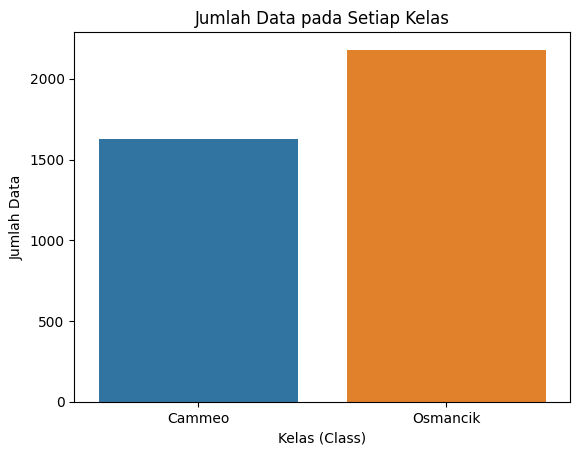
\includegraphics{Rice_PSD_files/figure-pdf/cell-9-output-1.png}

}

\end{figure}

\begin{verbatim}
Jumlah Data pada Setiap Kelas:
Osmancik    2180
Cammeo      1630
Name: Class, dtype: int64
\end{verbatim}

Pada distribusi class ini, terlihat bahwa class cameo memiliki data
sebanyak 1630 lebih sedikit dari pada class osmancik yaitu sebanyak 2180

\hypertarget{seleksi-fitur}{%
\subsection{Seleksi Fitur}\label{seleksi-fitur}}

Seleksi fitur adalah langkah penting dalam pemrosesan data untuk
meningkatkan kinerja model dan mengurangi overfitting. ANOVA (Analysis
of Variance) digunakan untuk mengukur perbedaan rata-rata antara dua
atau lebih kelompok. Dalam konteks ini, kita akan menggunakan ANOVA
untuk memilih fitur-fitur terbaik yang paling berpengaruh terhadap
klasifikasi jenis biji beras.

Langkah-langkah:

\begin{enumerate}
\def\labelenumi{\arabic{enumi}.}
\item
  Menentukan Banyaknya Fitur (N): Pertama, kita perlu menentukan jumlah
  total fitur dalam dataset.
\item
  Menentukan Jumlah Fitur Terbaik (K): Kita juga perlu menentukan jumlah
  fitur terbaik yang ingin kita pilih. Dalam contoh ini, K diatur
  menjadi 6.
\item
  Inisialisasi Selector: Menggunakan SelectKBest dari scikit-learn
  dengan fungsi skor ANOVA (f\_classif) dan jumlah fitur terbaik (K)
  yang telah ditentukan.
\end{enumerate}

\begin{Shaded}
\begin{Highlighting}[]


\CommentTok{\# Menentukan banyaknya fitur (N)}
\NormalTok{total\_features }\OperatorTok{=} \BuiltInTok{len}\NormalTok{(X.columns)}

\CommentTok{\# Menentukan jumlah fitur terbaik (K)}
\NormalTok{k\_best\_features }\OperatorTok{=} \DecValTok{6}

\CommentTok{\# Inisialisasi Selector}
\NormalTok{selector }\OperatorTok{=}\NormalTok{ SelectKBest(score\_func}\OperatorTok{=}\NormalTok{f\_classif, k}\OperatorTok{=}\NormalTok{k\_best\_features)}
\end{Highlighting}
\end{Shaded}

\begin{Shaded}
\begin{Highlighting}[]
\CommentTok{\# Lakukan seleksi fitur}
\NormalTok{selector.fit(X, y)}
\end{Highlighting}
\end{Shaded}

\begin{verbatim}
SelectKBest(k=6)
\end{verbatim}

\begin{Shaded}
\begin{Highlighting}[]
\CommentTok{\# Tampilkan hasil seleksi fitur}
\CommentTok{\# Jumlah fitur terbaik yang terpilih disesuaikan dengan nilai K di atas}
\NormalTok{selected\_features }\OperatorTok{=}\NormalTok{ selector.get\_support(indices}\OperatorTok{=}\VariableTok{True}\NormalTok{)}
\NormalTok{feature\_names }\OperatorTok{=}\NormalTok{ X.columns}

\CommentTok{\# Pilih nama{-}nama fitur yang dipilih}
\NormalTok{selected\_feature\_names }\OperatorTok{=}\NormalTok{ [feature\_names[i] }\ControlFlowTok{for}\NormalTok{ i }\KeywordTok{in}\NormalTok{ selected\_features]}

\CommentTok{\# Hitung skor statistik untuk setiap fitur}
\NormalTok{scores }\OperatorTok{=}\NormalTok{ selector.scores\_[selected\_features]}

\CommentTok{\# Membuat bar chart}
\NormalTok{plt.figure(figsize}\OperatorTok{=}\NormalTok{(}\DecValTok{10}\NormalTok{, }\DecValTok{6}\NormalTok{))}
\NormalTok{plt.bar(selected\_feature\_names, scores, color}\OperatorTok{=}\StringTok{\textquotesingle{}skyblue\textquotesingle{}}\NormalTok{)}
\NormalTok{plt.xlabel(}\StringTok{\textquotesingle{}Fitur\textquotesingle{}}\NormalTok{)}
\NormalTok{plt.ylabel(}\StringTok{\textquotesingle{}Skor Statistik\textquotesingle{}}\NormalTok{)}
\NormalTok{plt.title(}\StringTok{\textquotesingle{}Skor Statistik untuk Fitur{-}Fitur Terpilih\textquotesingle{}}\NormalTok{)}
\NormalTok{plt.xticks(rotation}\OperatorTok{=}\DecValTok{45}\NormalTok{)}
\NormalTok{plt.tight\_layout()}

\CommentTok{\# Menampilkan grafik}
\NormalTok{plt.show()}
\end{Highlighting}
\end{Shaded}

\begin{figure}[H]

{\centering 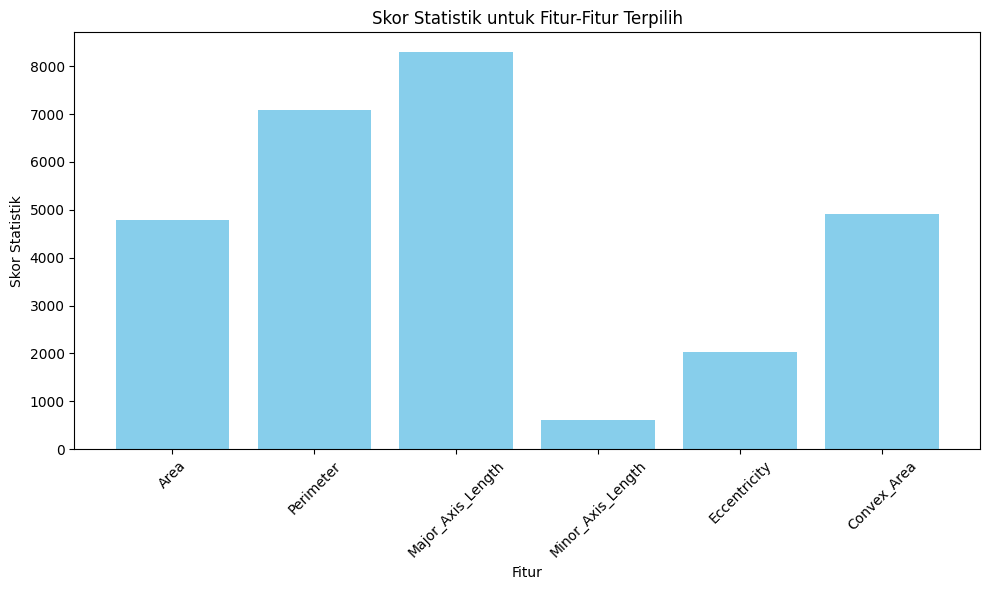
\includegraphics{Rice_PSD_files/figure-pdf/cell-12-output-1.png}

}

\end{figure}

\begin{Shaded}
\begin{Highlighting}[]
\CommentTok{\# Pilih hanya fitur{-}fitur terbaik}
\NormalTok{X\_selected }\OperatorTok{=}\NormalTok{ X[selected\_feature\_names]}
\end{Highlighting}
\end{Shaded}

Rumus ANOVA: \[
F = \frac{MSB}{MSW}
\] MSB atau mean square antar kelompok (mean square between groups).
dapat dari rumus ini :

\[
MSB = \frac{\sum_{i=1}^{k} n_i (\bar{X}_i - \bar{X}_{\text{total}})^2}{k - 1}
\] dan MSW atau mean square dalam kelompok (mean square within groups)

\[
MSW = \frac{\sum_{i=1}^{k} \sum_{j=1}^{n_i} (X_{ij} - \bar{X}_i)^2}{N - k}
\]

\begin{Shaded}
\begin{Highlighting}[]
\CommentTok{\# Menampilkan dataset yang sudah dipilih hanya dengan fitur{-}fitur terbaik}
\NormalTok{X\_selected.head()}
\end{Highlighting}
\end{Shaded}

\begin{longtable}[]{@{}lllllll@{}}
\toprule\noalign{}
& Area & Perimeter & Major\_Axis\_Length & Minor\_Axis\_Length &
Eccentricity & Convex\_Area \\
\midrule\noalign{}
\endhead
\bottomrule\noalign{}
\endlastfoot
0 & 15231 & 525.578979 & 229.749878 & 85.093788 & 0.928882 & 15617 \\
1 & 14656 & 494.311005 & 206.020065 & 91.730972 & 0.895405 & 15072 \\
2 & 14634 & 501.122009 & 214.106781 & 87.768288 & 0.912118 & 14954 \\
3 & 13176 & 458.342987 & 193.337387 & 87.448395 & 0.891861 & 13368 \\
4 & 14688 & 507.166992 & 211.743378 & 89.312454 & 0.906691 & 15262 \\
\end{longtable}

untuk membuang fitur yang skor statistik nya rendah

\hypertarget{preprocesing-data}{%
\section{Preprocesing Data}\label{preprocesing-data}}

\hypertarget{split-data}{%
\subsection{Split data}\label{split-data}}

\begin{Shaded}
\begin{Highlighting}[]
\ImportTok{from}\NormalTok{ sklearn.model\_selection }\ImportTok{import}\NormalTok{ train\_test\_split}

\CommentTok{\# Pembagian data menjadi data latih dan data uji (80\% data latih, 20\% data uji)}
\NormalTok{X\_train, X\_test, y\_train, y\_test }\OperatorTok{=}\NormalTok{ train\_test\_split(X\_selected, y, test\_size}\OperatorTok{=}\FloatTok{0.2}\NormalTok{, random\_state}\OperatorTok{=}\DecValTok{42}\NormalTok{)}
\end{Highlighting}
\end{Shaded}

\begin{Shaded}
\begin{Highlighting}[]
\NormalTok{X\_train.shape}
\end{Highlighting}
\end{Shaded}

\begin{verbatim}
(3048, 6)
\end{verbatim}

\begin{Shaded}
\begin{Highlighting}[]
\NormalTok{y\_train}
\end{Highlighting}
\end{Shaded}

\begin{verbatim}
3644    Osmancik
3418    Osmancik
1351      Cammeo
3591    Osmancik
246       Cammeo
          ...   
1130      Cammeo
1294      Cammeo
860       Cammeo
3507    Osmancik
3174    Osmancik
Name: Class, Length: 3048, dtype: object
\end{verbatim}

\hypertarget{normalisasi-data}{%
\subsection{Normalisasi Data}\label{normalisasi-data}}

Normalisasi data dengan Min-Max Scaling adalah suatu teknik transformasi
pada data numerik sehingga nilai-nilai tersebut dapat diubah ke dalam
rentang yang lebih kecil, biasanya antara 0 dan 1. Rumus Min-Max Scaling
untuk suatu nilai (x) dalam rentang asal ({[}a, b{]}) menjadi nilai
dalam rentang baru ({[}c, d{]}) adalah sebagai berikut: \[
\
\text{Scaled Value} = \frac{x - a}{b - a} \times (d - c) + c
\
\] Dengan penjelasan sebagai berikut:

\begin{itemize}
\tightlist
\item
  (x) adalah nilai asli dari fitur.
\item
  (a) adalah nilai minimum dalam rentang asal.
\item
  (b) adalah nilai maksimum dalam rentang asal.
\item
  (c) adalah nilai minimum dalam rentang baru.
\item
  (d) adalah nilai maksimum dalam rentang baru.
\end{itemize}

Proses normalisasi ini akan membantu mencegah perbedaan skala antar
fitur, yang dapat meningkatkan performa model machine learning, terutama
untuk model-model yang sensitif terhadap skala seperti Support Vector
Machines (SVM) atau k-Nearest Neighbors (kNN).

\begin{Shaded}
\begin{Highlighting}[]
\CommentTok{\# Normalisasi data}
\NormalTok{scaler }\OperatorTok{=}\NormalTok{ MinMaxScaler()}
\NormalTok{X\_train\_scaled }\OperatorTok{=}\NormalTok{ scaler.fit\_transform(X\_train)}
\NormalTok{X\_test\_scaled }\OperatorTok{=}\NormalTok{ scaler.transform(X\_test)}
\end{Highlighting}
\end{Shaded}

\hypertarget{modelling}{%
\section{Modelling}\label{modelling}}

\hypertarget{support-vector-machine-svm}{%
\subsection{Support Vector Machine
(SVM)}\label{support-vector-machine-svm}}

Support Vector Machine (SVM) adalah model klasifikasi yang mencoba
menemukan hyperplane terbaik yang memisahkan dua kelas dalam ruang
fitur. Fungsi keputusan SVM dapat dinyatakan sebagai:

\[
f(x) = \text{sign}(\mathbf{w} \cdot \mathbf{x} + b)
\]

\begin{itemize}
\tightlist
\item
  \(\mathbf{w}\) adalah vektor bobot,
\item
  \(\mathbf{x}\) adalah vektor fitur input,
\item
  \(b\) adalah bias, dan
\item
  \(\text{sign}\) adalah fungsi tanda.
\end{itemize}

\begin{Shaded}
\begin{Highlighting}[]
\ImportTok{from}\NormalTok{ sklearn.svm }\ImportTok{import}\NormalTok{ SVC}
\ImportTok{from}\NormalTok{ sklearn.metrics }\ImportTok{import}\NormalTok{ accuracy\_score, classification\_report, confusion\_matrix}

\CommentTok{\# Inisialisasi model SVM}
\NormalTok{svm\_model }\OperatorTok{=}\NormalTok{ SVC(kernel}\OperatorTok{=}\StringTok{\textquotesingle{}linear\textquotesingle{}}\NormalTok{, random\_state}\OperatorTok{=}\DecValTok{42}\NormalTok{)}

\CommentTok{\# Latih model SVM}
\NormalTok{svm\_model.fit(X\_train\_scaled, y\_train)}

\CommentTok{\# Prediksi data uji}
\NormalTok{svm\_predictions }\OperatorTok{=}\NormalTok{ svm\_model.predict(X\_test\_scaled)}

\CommentTok{\# Evaluasi model}
\NormalTok{svm\_accuracy }\OperatorTok{=}\NormalTok{ accuracy\_score(y\_test, svm\_predictions)}
\NormalTok{svm\_classification\_report }\OperatorTok{=}\NormalTok{ classification\_report(y\_test, svm\_predictions)}
\NormalTok{svm\_confusion\_matrix }\OperatorTok{=}\NormalTok{ confusion\_matrix(y\_test, svm\_predictions)}

\CommentTok{\# Tampilkan hasil evaluasi}
\BuiltInTok{print}\NormalTok{(}\SpecialStringTok{f\textquotesingle{}Accuracy of SVM: }\SpecialCharTok{\{}\NormalTok{svm\_accuracy}\SpecialCharTok{\}}\SpecialStringTok{\textquotesingle{}}\NormalTok{)}
\end{Highlighting}
\end{Shaded}

\begin{verbatim}
Accuracy of SVM: 0.931758530183727
\end{verbatim}

\hypertarget{random-forest}{%
\subsection{Random Forest}\label{random-forest}}

Random Forest adalah model ensemble yang terdiri dari sejumlah besar
pohon keputusan. Prediksi dari Random Forest diperoleh dengan
menggabungkan prediksi dari setiap pohon. Fungsi keputusan Random Forest
dapat dinyatakan sebagai:

\[
f(x) = \text{mode}(f_1(x), f_2(x), ..., f_N(x))
\]

\begin{itemize}
\tightlist
\item
  \(f_i(x)\) adalah fungsi keputusan pohon ke-\(i\), dan
\item
  \(\text{mode}\) adalah modus dari prediksi semua pohon.
\end{itemize}

\begin{Shaded}
\begin{Highlighting}[]
\ImportTok{from}\NormalTok{ sklearn.ensemble }\ImportTok{import}\NormalTok{ RandomForestClassifier}

\CommentTok{\# Inisialisasi model Random Forest}
\NormalTok{rf\_model }\OperatorTok{=}\NormalTok{ RandomForestClassifier(n\_estimators}\OperatorTok{=}\DecValTok{100}\NormalTok{, random\_state}\OperatorTok{=}\DecValTok{42}\NormalTok{)}

\CommentTok{\# Latih model Random Forest}
\NormalTok{rf\_model.fit(X\_train\_scaled, y\_train)}

\CommentTok{\# Prediksi data uji}
\NormalTok{rf\_predictions }\OperatorTok{=}\NormalTok{ rf\_model.predict(X\_test\_scaled)}

\CommentTok{\# Evaluasi model}
\NormalTok{rf\_accuracy }\OperatorTok{=}\NormalTok{ accuracy\_score(y\_test, rf\_predictions)}
\NormalTok{rf\_classification\_report }\OperatorTok{=}\NormalTok{ classification\_report(y\_test, rf\_predictions)}
\NormalTok{rf\_confusion\_matrix }\OperatorTok{=}\NormalTok{ confusion\_matrix(y\_test, rf\_predictions)}

\CommentTok{\# Tampilkan hasil evaluasi}
\BuiltInTok{print}\NormalTok{(}\SpecialStringTok{f\textquotesingle{}Accuracy of Random Forest: }\SpecialCharTok{\{}\NormalTok{rf\_accuracy}\SpecialCharTok{\}}\SpecialStringTok{\textquotesingle{}}\NormalTok{)}
\end{Highlighting}
\end{Shaded}

\begin{verbatim}
Accuracy of Random Forest: 0.916010498687664
\end{verbatim}

\hypertarget{neural-network}{%
\subsection{Neural Network}\label{neural-network}}

Jaringan Saraf Tiruan (Neural Network) adalah model yang terdiri dari
lapisan-lapisan neuron yang saling terhubung. Fungsi keputusan untuk
jaringan saraf tiruan dapat dinyatakan sebagai:

\[
f(x) = \text{softmax}(\mathbf{W}_2 \cdot \text{ReLU}(\mathbf{W}_1 \cdot \mathbf{x} + \mathbf{b}_1) + \mathbf{b}_2)
\]

\begin{itemize}
\tightlist
\item
  \(\mathbf{W}_1\) dan \(\mathbf{W}_2\) adalah matriks bobot,
\item
  \(\mathbf{b}_1\) dan \(\mathbf{b}_2\) adalah vektor bias,
\item
  \(\mathbf{x}\) adalah vektor fitur input,
\item
  \(\text{ReLU}\) adalah fungsi aktivasi ReLU, dan
\item
  \(\text{softmax}\) adalah fungsi aktivasi softmax.
\end{itemize}

\begin{Shaded}
\begin{Highlighting}[]
\ImportTok{from}\NormalTok{ sklearn.neural\_network }\ImportTok{import}\NormalTok{ MLPClassifier}

\CommentTok{\# Inisialisasi model Neural Network}
\NormalTok{nn\_model }\OperatorTok{=}\NormalTok{ MLPClassifier(hidden\_layer\_sizes}\OperatorTok{=}\NormalTok{(}\DecValTok{64}\NormalTok{, }\DecValTok{32}\NormalTok{), max\_iter}\OperatorTok{=}\DecValTok{1000}\NormalTok{, random\_state}\OperatorTok{=}\DecValTok{42}\NormalTok{)}

\CommentTok{\# Latih model Neural Network}
\NormalTok{nn\_model.fit(X\_train\_scaled, y\_train)}

\CommentTok{\# Prediksi data uji}
\NormalTok{nn\_predictions }\OperatorTok{=}\NormalTok{ nn\_model.predict(X\_test\_scaled)}

\CommentTok{\# Evaluasi model}
\NormalTok{nn\_accuracy }\OperatorTok{=}\NormalTok{ accuracy\_score(y\_test, nn\_predictions)}
\NormalTok{nn\_classification\_report }\OperatorTok{=}\NormalTok{ classification\_report(y\_test, nn\_predictions)}
\NormalTok{nn\_confusion\_matrix }\OperatorTok{=}\NormalTok{ confusion\_matrix(y\_test, nn\_predictions)}

\CommentTok{\# Tampilkan hasil evaluasi}
\BuiltInTok{print}\NormalTok{(}\SpecialStringTok{f\textquotesingle{}Accuracy of Neural Network: }\SpecialCharTok{\{}\NormalTok{nn\_accuracy}\SpecialCharTok{\}}\SpecialStringTok{\textquotesingle{}}\NormalTok{)}
\end{Highlighting}
\end{Shaded}

\begin{verbatim}
Accuracy of Neural Network: 0.9278215223097113
\end{verbatim}

\hypertarget{evaluasi}{%
\section{Evaluasi}\label{evaluasi}}

Akurasi yang tertinggi yang saya dapat dari hasil yang sudah dibuat
adalah SVM

\begin{Shaded}
\begin{Highlighting}[]
\BuiltInTok{print}\NormalTok{(}\StringTok{"Accuracy of SVM:"}\NormalTok{,svm\_accuracy)}
\BuiltInTok{print}\NormalTok{(}\StringTok{"Accuracy of Random Forest:"}\NormalTok{, rf\_accuracy)}
\BuiltInTok{print}\NormalTok{(}\StringTok{"Accuracy of Neural Network:"}\NormalTok{, nn\_accuracy)}
\end{Highlighting}
\end{Shaded}

\begin{verbatim}
Accuracy of SVM: 0.931758530183727
Accuracy of Random Forest: 0.916010498687664
Accuracy of Neural Network: 0.9278215223097113
\end{verbatim}

\begin{Shaded}
\begin{Highlighting}[]
\ImportTok{import}\NormalTok{ matplotlib.pyplot }\ImportTok{as}\NormalTok{ plt}

\CommentTok{\# Data akurasi}
\NormalTok{models }\OperatorTok{=}\NormalTok{ [}\StringTok{\textquotesingle{}SVM\textquotesingle{}}\NormalTok{, }\StringTok{\textquotesingle{}Random Forest\textquotesingle{}}\NormalTok{, }\StringTok{\textquotesingle{}Neural Network\textquotesingle{}}\NormalTok{]}
\NormalTok{accuracies }\OperatorTok{=}\NormalTok{ [svm\_accuracy, rf\_accuracy, nn\_accuracy]}

\CommentTok{\# Membuat diagram batang}
\NormalTok{plt.figure(figsize}\OperatorTok{=}\NormalTok{(}\DecValTok{10}\NormalTok{, }\DecValTok{6}\NormalTok{))}
\NormalTok{plt.bar(models, accuracies, color}\OperatorTok{=}\NormalTok{[}\StringTok{\textquotesingle{}blue\textquotesingle{}}\NormalTok{, }\StringTok{\textquotesingle{}orange\textquotesingle{}}\NormalTok{, }\StringTok{\textquotesingle{}green\textquotesingle{}}\NormalTok{, }\StringTok{\textquotesingle{}purple\textquotesingle{}}\NormalTok{])}
\NormalTok{plt.ylim(}\DecValTok{0}\NormalTok{, }\DecValTok{1}\NormalTok{)  }\CommentTok{\# Menetapkan batas y{-}axis antara 0 dan 1}
\NormalTok{plt.title(}\StringTok{\textquotesingle{}Akurasi Model Klasifikasi\textquotesingle{}}\NormalTok{)}
\NormalTok{plt.xlabel(}\StringTok{\textquotesingle{}Model\textquotesingle{}}\NormalTok{)}
\NormalTok{plt.ylabel(}\StringTok{\textquotesingle{}Akurasi\textquotesingle{}}\NormalTok{)}
\NormalTok{plt.show()}
\end{Highlighting}
\end{Shaded}

\begin{figure}[H]

{\centering 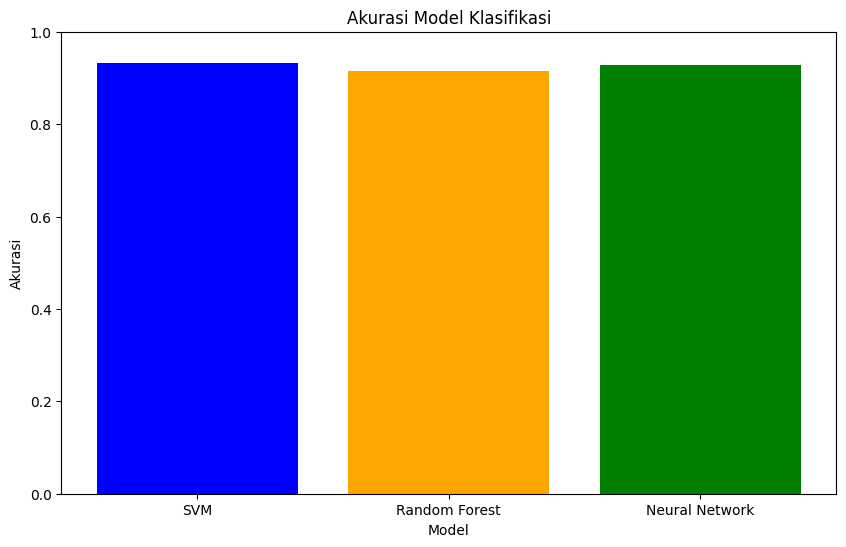
\includegraphics{Rice_PSD_files/figure-pdf/cell-24-output-1.png}

}

\end{figure}

Save Model

\begin{Shaded}
\begin{Highlighting}[]
\ImportTok{import}\NormalTok{ joblib}
\NormalTok{joblib.dump(svm\_model, }\StringTok{\textquotesingle{}/content/drive/MyDrive/Proyek Sain Data/Model/svm\_model.pkl\textquotesingle{}}\NormalTok{)}
\end{Highlighting}
\end{Shaded}

\begin{verbatim}
['/content/drive/MyDrive/Proyek Sain Data/Model/svm_model.pkl']
\end{verbatim}

\bookmarksetup{startatroot}

\hypertarget{summary}{%
\chapter{Summary}\label{summary}}

In summary, this book has no content whatsoever.

\bookmarksetup{startatroot}

\hypertarget{references}{%
\chapter*{References}\label{references}}
\addcontentsline{toc}{chapter}{References}

\markboth{References}{References}

\hypertarget{refs}{}
\begin{CSLReferences}{0}{0}
\end{CSLReferences}



\backmatter
\printindex

\end{document}
